\documentclass{beamer}
\usepackage{graphicx,url}
\usepackage[brazil]{babel}   
\usepackage[utf8]{inputenc}
\usepackage{pgf,tikz}
\usepackage{adjustbox}
\usepackage{mathrsfs}
\usepackage{listings}
\usetikzlibrary{calc}
\usetikzlibrary{arrows}
\batchmode
\usepackage{amsmath,amssymb,enumerate,epsfig,bbm,calc,color,ifthen,capt-of}
\usetheme{Berlin}
%-------------------------Titulo/Autores/Orientador------------------------------------------------
\title[Fast Obstacle k-Nearest Neighbour Query on Navigation Mesh]{
    Fast Obstacle k-Nearest Neighbour Query on Navigation Mesh \\
}
\subtitle {Final Presentation}
\date{}
\author[Shizhe Zhao]{
    Shizhe Zhao (27505928)\\
    Supervisors: David Taniar, Daniel Harabor
}

\pgfdeclareimage[height=0.7cm]{monash-logo}{MonashCrest.pdf}
\logo{\pgfuseimage{monash-logo}\hspace*{0.5cm}}

\AtBeginSection[]
{
  \begin{frame}<beamer>
    \frametitle{Outline}
    \tableofcontents[currentsection]
  \end{frame}
}
\setbeamercovered{transparent}
\beamerdefaultoverlayspecification{<+->}
% -----------------------------------------------------------------------------
\begin{document}
% -----------------------------------------------------------------------------

%---Summary---------------------------------------------------------
\frame{\titlepage}
\section[]{}
% \begin{frame}{Summary}
%   \tableofcontents
% \end{frame}

\section{Introduction}
\begin{frame}{Traditional k-Nearest Neighbor}
\setbeamercovered{invisible}
\begin{minipage}{.5\textwidth}
\small k-Nearest Neighbor:
\begin{itemize}
    \item<1-> \small Given:
    \begin{itemize}
        \item<2-> \small $q$: query point
        \item<3-> \small $T$: target set\\\tiny(e.g. $\{A,B,C,D\}$)
        \item<4-> \small $k$: number of retrieved targets \tiny(e.g. $k=1$)
    \end{itemize}
    \item<5-> \small Return:\\top $k$ targets regarding \textit{Euclidean distance}
    \item<6-> \small the circle indicates that $D$ is the nearest neighbor of $q$
\end{itemize}
\end{minipage}%
\begin{minipage}{.5\textwidth}
\begin{adjustbox}{max totalsize={.9\textwidth}{.9\textheight}, right}
\begin{tikzpicture}[line cap=round,line join=round,>=triangle 45,x=1.0cm,y=1.0cm]
\definecolor{aqaqaq}{rgb}{0.6274509803921569,0.6274509803921569,0.6274509803921569}
\definecolor{qqqqff}{rgb}{0.,0.,1.}
\definecolor{ffqqqq}{rgb}{1.,0.,0.}
\clip(3.5,-2.7) rectangle (10.5,2.5);
\draw [line width=1.2pt,dash pattern=on 1pt off 1pt,color=aqaqaq,fill=aqaqaq,fill opacity=0.30000001192092896] (6.965791019668495,-0.8590646710374431) circle (1.226394681592311cm);
\begin{scriptsize}
\draw [fill=ffqqqq] (6.965791019668495,-0.8590646710374431) circle (2.5pt);
\draw[color=ffqqqq] (7.1713402737586955,-0.4852111547881992) node {$q$};
\draw [fill=qqqqff] (3.786645549990551,1.7424425037681481) circle (2.5pt);
\draw[color=qqqqff] (3.8990767613748694,2.0486954624936313) node {$A$};
\draw [fill=qqqqff] (7.240860537026145,0.8341118960661955) circle (2.5pt);
\draw[color=qqqqff] (7.355929497534194,1.1425301821411886) node {$B$};
\draw [fill=qqqqff] (6.786032179750889,-2.084374701009021) circle (2.5pt);
\draw[color=qqqqff] (6.5840109253821115,-2.4150075851684014) node {$D$};
\draw [fill=qqqqff] (8.744888255475496,0.3259148131345835) circle (2.5pt);
\draw[color=qqqqff] (8.866204964788267,0.6391050263898316) node {$C$};
\end{scriptsize}
\end{tikzpicture}
\end{adjustbox}
\end{minipage}
\end{frame}

\begin{frame}{Obstacle k-Nearest Neighbor}
\begin{minipage}{.5\textwidth}
\begin{itemize}
    \item \small traditional kNN has been well studied.
    \item \small when take obstacles into consideration...
\end{itemize}
\end{minipage}%
\begin{minipage}{.5\textwidth}
\begin{adjustbox}{max totalsize={.9\textwidth}{.9\textheight}, right}
\only<1,2> {\begin{tikzpicture}[line cap=round,line join=round,>=triangle 45,x=1.0cm,y=1.0cm]
\definecolor{aqaqaq}{rgb}{0.6274509803921569,0.6274509803921569,0.6274509803921569}
\definecolor{qqqqff}{rgb}{0.,0.,1.}
\definecolor{ffqqqq}{rgb}{1.,0.,0.}
\clip(3.5,-2.7) rectangle (10.5,2.5);
\draw [line width=1.2pt,dash pattern=on 1pt off 1pt,color=aqaqaq,fill=aqaqaq,fill opacity=0.30000001192092896] (6.965791019668495,-0.8590646710374431) circle (1.226394681592311cm);
\begin{scriptsize}
\draw [fill=ffqqqq] (6.965791019668495,-0.8590646710374431) circle (2.5pt);
\draw[color=ffqqqq] (7.1713402737586955,-0.4852111547881992) node {$q$};
\draw [fill=qqqqff] (3.786645549990551,1.7424425037681481) circle (2.5pt);
\draw[color=qqqqff] (3.8990767613748694,2.0486954624936313) node {$A$};
\draw [fill=qqqqff] (7.240860537026145,0.8341118960661955) circle (2.5pt);
\draw[color=qqqqff] (7.355929497534194,1.1425301821411886) node {$B$};
\draw [fill=qqqqff] (6.786032179750889,-2.084374701009021) circle (2.5pt);
\draw[color=qqqqff] (6.5840109253821115,-2.4150075851684014) node {$D$};
\draw [fill=qqqqff] (8.744888255475496,0.3259148131345835) circle (2.5pt);
\draw[color=qqqqff] (8.866204964788267,0.6391050263898316) node {$C$};
\end{scriptsize}
\end{tikzpicture}}
\only<3-> {\begin{tikzpicture}[line cap=round,line join=round,>=triangle 45,x=1.0cm,y=1.0cm]
\definecolor{aqaqaq}{rgb}{0.6274509803921569,0.6274509803921569,0.6274509803921569}
\definecolor{qqqqff}{rgb}{0.,0.,1.}
\definecolor{ffqqqq}{rgb}{1.,0.,0.}

\clip(3.5,-2.7) rectangle (10.5,2.5);
\fill[line width=1.2pt,fill=black,fill opacity=0.8999999761581421] (4.273473007276684,-0.8915497346423199) -- (4.311125781159042,-1.6311118832188969) -- (10.071125781159033,-1.891111883218897) -- (10.011125781159034,-1.231111883218897) -- cycle;
\fill[line width=1.2pt,fill=black,fill opacity=1.0] (6.370910095846811,0.5910375080896166) -- (6.434877040051173,0.002541621409478362) -- (8.639743589985672,-0.6535907548495615) -- (8.748484255211462,0.3402661877139281) -- cycle;
\draw [line width=1.2pt,dash pattern=on 1pt off 1pt,color=aqaqaq,fill=aqaqaq,fill opacity=0.30000001192092896] (6.965791019668495,-0.8590646710374431) circle (1.226394681592311cm);
\draw [line width=1.2pt] (8.63151379877438,-0.6620475590162423)-- (8.744888255475496,0.3259148131345835);
\draw [line width=1.2pt] (6.965791019668495,-0.8590646710374431)-- (6.436308033635486,-0.035167994675882754);
\draw [line width=1.2pt] (6.965791019668495,-0.8590646710374431)-- (3.786645549990551,1.7424425037681481);
\draw [line width=1.2pt] (6.965791019668495,-0.8590646710374431)-- (4.274665113870528,-0.9032956187025807);
\draw [line width=1.2pt] (4.274665113870528,-0.9032956187025807)-- (4.306017252514734,-1.6439597133614232);
\draw [line width=1.2pt] (4.306017252514734,-1.6439597133614232)-- (6.786032179750889,-2.084374701009021);
\draw [line width=1.2pt] (6.434877040051173,0.002541621409478362)-- (6.370910095846811,0.5910375080896166);
\draw [line width=1.2pt] (6.370910095846811,0.5910375080896166)-- (7.240860537026145,0.8341118960661955);
\draw [line width=1.2pt] (6.965791019668495,-0.8590646710374431)-- (8.639743589985672,-0.6535907548495615);
\begin{scriptsize}
\draw [fill=ffqqqq] (6.965791019668495,-0.8590646710374431) circle (2.5pt);
\draw[color=ffqqqq] (7.1713402737586955,-0.4852111547881992) node {$q$};
\draw [fill=qqqqff] (3.786645549990551,1.7424425037681481) circle (2.5pt);
\draw[color=qqqqff] (3.8990767613748694,2.0486954624936313) node {$A$};
\draw [fill=qqqqff] (7.240860537026145,0.8341118960661955) circle (2.5pt);
\draw[color=qqqqff] (7.355929497534194,1.1425301821411886) node {$B$};
\draw [fill=qqqqff] (6.786032179750889,-2.084374701009021) circle (2.5pt);
\draw[color=qqqqff] (6.5840109253821115,-2.4150075851684014) node {$D$};
\draw [fill=qqqqff] (4.273473007276684,-0.8915497346423199) circle (2.5pt);
\draw [fill=qqqqff] (4.311125781159042,-1.6311118832188969) circle (2.5pt);
\draw [fill=qqqqff] (10.071125781159033,-1.891111883218897) circle (2.5pt);
\draw [fill=qqqqff] (10.011125781159034,-1.231111883218897) circle (2.5pt);
\draw [fill=qqqqff] (6.370910095846811,0.5910375080896166) circle (2.5pt);
\draw [fill=qqqqff] (6.434877040051173,0.002541621409478362) circle (2.5pt);
\draw [fill=qqqqff] (8.639743589985672,-0.6535907548495615) circle (2.5pt);
\draw [fill=qqqqff] (8.744888255475496,0.3259148131345835) circle (2.5pt);
\draw[color=qqqqff] (8.866204964788267,0.6391050263898316) node {$C$};
\end{scriptsize}
\end{tikzpicture}}
\end{adjustbox}
\end{minipage}
\end{frame}

\begin{frame}{Application Scenario}
\begin{minipage}{.5\textwidth}
\small In an industrial warehouse,\\
{\color{red}$q$} is a robot.\\
It's interested in the closest storage locations,\\
but it can not cross obstacles
\end{minipage}%
\begin{minipage}{.5\textwidth}
\begin{adjustbox}{max totalsize={.9\textwidth}{.9\textheight}, right}
\begin{tikzpicture}[line cap=round,line join=round,>=triangle 45,x=1.0cm,y=1.0cm]
\definecolor{aqaqaq}{rgb}{0.6274509803921569,0.6274509803921569,0.6274509803921569}
\definecolor{qqqqff}{rgb}{0.,0.,1.}
\definecolor{ffqqqq}{rgb}{1.,0.,0.}

\clip(3.5,-2.7) rectangle (10.5,2.5);
\fill[line width=1.2pt,fill=black,fill opacity=0.8999999761581421] (4.273473007276684,-0.8915497346423199) -- (4.311125781159042,-1.6311118832188969) -- (10.071125781159033,-1.891111883218897) -- (10.011125781159034,-1.231111883218897) -- cycle;
\fill[line width=1.2pt,fill=black,fill opacity=1.0] (6.370910095846811,0.5910375080896166) -- (6.434877040051173,0.002541621409478362) -- (8.639743589985672,-0.6535907548495615) -- (8.748484255211462,0.3402661877139281) -- cycle;
\draw [line width=1.2pt,dash pattern=on 1pt off 1pt,color=aqaqaq,fill=aqaqaq,fill opacity=0.30000001192092896] (6.965791019668495,-0.8590646710374431) circle (1.226394681592311cm);
\draw [line width=1.2pt] (8.63151379877438,-0.6620475590162423)-- (8.744888255475496,0.3259148131345835);
\draw [line width=1.2pt] (6.965791019668495,-0.8590646710374431)-- (6.436308033635486,-0.035167994675882754);
\draw [line width=1.2pt] (6.965791019668495,-0.8590646710374431)-- (3.786645549990551,1.7424425037681481);
\draw [line width=1.2pt] (6.965791019668495,-0.8590646710374431)-- (4.274665113870528,-0.9032956187025807);
\draw [line width=1.2pt] (4.274665113870528,-0.9032956187025807)-- (4.306017252514734,-1.6439597133614232);
\draw [line width=1.2pt] (4.306017252514734,-1.6439597133614232)-- (6.786032179750889,-2.084374701009021);
\draw [line width=1.2pt] (6.434877040051173,0.002541621409478362)-- (6.370910095846811,0.5910375080896166);
\draw [line width=1.2pt] (6.370910095846811,0.5910375080896166)-- (7.240860537026145,0.8341118960661955);
\draw [line width=1.2pt] (6.965791019668495,-0.8590646710374431)-- (8.639743589985672,-0.6535907548495615);
\begin{scriptsize}
\draw [fill=ffqqqq] (6.965791019668495,-0.8590646710374431) circle (2.5pt);
\draw[color=ffqqqq] (7.1713402737586955,-0.4852111547881992) node {$q$};
\draw [fill=qqqqff] (3.786645549990551,1.7424425037681481) circle (2.5pt);
\draw[color=qqqqff] (3.8990767613748694,2.0486954624936313) node {$A$};
\draw [fill=qqqqff] (7.240860537026145,0.8341118960661955) circle (2.5pt);
\draw[color=qqqqff] (7.355929497534194,1.1425301821411886) node {$B$};
\draw [fill=qqqqff] (6.786032179750889,-2.084374701009021) circle (2.5pt);
\draw[color=qqqqff] (6.5840109253821115,-2.4150075851684014) node {$D$};
\draw [fill=qqqqff] (4.273473007276684,-0.8915497346423199) circle (2.5pt);
\draw [fill=qqqqff] (4.311125781159042,-1.6311118832188969) circle (2.5pt);
\draw [fill=qqqqff] (10.071125781159033,-1.891111883218897) circle (2.5pt);
\draw [fill=qqqqff] (10.011125781159034,-1.231111883218897) circle (2.5pt);
\draw [fill=qqqqff] (6.370910095846811,0.5910375080896166) circle (2.5pt);
\draw [fill=qqqqff] (6.434877040051173,0.002541621409478362) circle (2.5pt);
\draw [fill=qqqqff] (8.639743589985672,-0.6535907548495615) circle (2.5pt);
\draw [fill=qqqqff] (8.744888255475496,0.3259148131345835) circle (2.5pt);
\draw[color=qqqqff] (8.866204964788267,0.6391050263898316) node {$C$};
\end{scriptsize}
\end{tikzpicture}
\end{adjustbox}
\end{minipage}
\end{frame}
\section{Related works}
\begin{frame}{How to compute Obstacle Distance}
\begin{minipage}{.4\textwidth}
\begin{itemize}
\item \small Existing works rely on \textit{visibility graph} (VG)
    \begin{itemize}
        \item \small any pair of visible points has an edge
    \end{itemize}
\item \small Run shortest path algorithm on \textit{VG}\\
    \tiny{(e.g. \textit{Dijkstra})}
\item \small {Number of edge: up to $O(V^2)$\\
            \tiny{($V$: the number of vertex})}
\end{itemize}
\end{minipage}%
\begin{minipage}{.6\textwidth}
\begin{adjustbox}{max totalsize={.9\textwidth}{.9\textheight}, right}
\begin{tikzpicture}
    \newcommand{\nodelabel}[2] {
    \fill[red] (#1) circle[radius=.5ex];
    \node[#2] at (#1) {#1};
}

\newcommand{\medge}[2]{
    \draw[gray,thick] (#1)--(#2);
}

\newcommand{\drawVs}{
    %\nodelabel{a}{above}
    \nodelabel{b}{below}
    \nodelabel{c}{below}
    
    %\nodelabel{d}{left}
    \nodelabel{e}{right}
    \nodelabel{f}{below}
    
    \nodelabel{g}{above}
    \nodelabel{h}{below}
    %\nodelabel{i}{below}
}

\newcommand{\drawmeshs}{
    \medge{a}{k},\medge{a}{d},\medge{a}{b},\medge{a}{c}
    \medge{b}{c},
    \medge{c}{g}
    \medge{d}{f},\medge{d}{l},\medge{d}{e}
    \medge{l}{f}
    \medge{e}{c},\medge{e}{f}
    \medge{f}{h}
    \medge{g}{h},\medge{g}{b}
    \medge{h}{i}
}

\newcommand{\drawobstacles}{
    \fill[black] (a)--(b)--(c)--cycle;
    \fill[black] (g)--(h)--(i)--cycle;
    \fill[black] (d)--(e)--(f)--cycle;
}

%\coordinate (a) at (2, 6); 
\coordinate (a) at (0, 7);
\coordinate (b) at (8, 7); 
\coordinate (c) at (6, 5); 
\coordinate (d) at (1, 3);
\coordinate (e) at (4, 3);
\coordinate (f) at (4, 2);
\coordinate (g) at (7, 4);
\coordinate (h) at (7, 2);
%\coordinate (i) at (9, 0);
\coordinate (i) at (10, 0);
\coordinate (j) at (5, 2);
\coordinate (k) at (0, 7);
\coordinate (l) at (0, 0);
\coordinate (m) at (10, 0);
\coordinate (n) at (10, 7);
\coordinate (q) at (3, 4);
\coordinate (t) at (9, 3); 
% boundary
\draw[black, ultra thick] (k)--(n)--(m)--(l)--cycle;

% obstacles
\drawobstacles
% mesh
\drawmeshs
% vertices
\drawVs
% start
\fill[blue] (q) circle[radius=.5ex];
\node[above] at (q) {$q$};
% end
\fill[blue] (t) circle[radius=.5ex];
\node[above] at (t) {$t$};
    \onslide<1->{\drawboundary}
    \onslide<1->{\drawobstacles}
    \onslide<2->{\drawVG}
\end{tikzpicture}
\end{adjustbox}
\end{minipage}
\end{frame}

\begin{frame}{How to compute Obstacle Distance}
\begin{minipage}{.4\textwidth}
\begin{itemize}
\item \small Global VG: expansive
\item \small Motivation: only consider query related area
\item \small {\textit{Zhang, EDBT 2004}: \textit{Local Visibility Graph (LVG)}}
\end{itemize}
\end{minipage}%
\begin{minipage}{.6\textwidth}
\begin{adjustbox}{max totalsize={.9\textwidth}{.9\textheight}, right}
\begin{tikzpicture}
    \newcommand{\nodelabel}[2] {
    \fill[red] (#1) circle[radius=.5ex];
    \node[#2] at (#1) {#1};
}

\newcommand{\medge}[2]{
    \draw[gray,thick] (#1)--(#2);
}

\newcommand{\drawVs}{
    %\nodelabel{a}{above}
    \nodelabel{b}{below}
    \nodelabel{c}{below}
    
    %\nodelabel{d}{left}
    \nodelabel{e}{right}
    \nodelabel{f}{below}
    
    \nodelabel{g}{above}
    \nodelabel{h}{below}
    %\nodelabel{i}{below}
}

\newcommand{\drawmeshs}{
    \medge{a}{k},\medge{a}{d},\medge{a}{b},\medge{a}{c}
    \medge{b}{c},
    \medge{c}{g}
    \medge{d}{f},\medge{d}{l},\medge{d}{e}
    \medge{l}{f}
    \medge{e}{c},\medge{e}{f}
    \medge{f}{h}
    \medge{g}{h},\medge{g}{b}
    \medge{h}{i}
}

\newcommand{\drawobstacles}{
    \fill[black] (a)--(b)--(c)--cycle;
    \fill[black] (g)--(h)--(i)--cycle;
    \fill[black] (d)--(e)--(f)--cycle;
}

%\coordinate (a) at (2, 6); 
\coordinate (a) at (0, 7);
\coordinate (b) at (8, 7); 
\coordinate (c) at (6, 5); 
\coordinate (d) at (1, 3);
\coordinate (e) at (4, 3);
\coordinate (f) at (4, 2);
\coordinate (g) at (7, 4);
\coordinate (h) at (7, 2);
%\coordinate (i) at (9, 0);
\coordinate (i) at (10, 0);
\coordinate (j) at (5, 2);
\coordinate (k) at (0, 7);
\coordinate (l) at (0, 0);
\coordinate (m) at (10, 0);
\coordinate (n) at (10, 7);
\coordinate (q) at (3, 4);
\coordinate (t) at (9, 3); 
% boundary
\draw[black, ultra thick] (k)--(n)--(m)--(l)--cycle;

% obstacles
\drawobstacles
% mesh
\drawmeshs
% vertices
\drawVs
% start
\fill[blue] (q) circle[radius=.5ex];
\node[above] at (q) {$q$};
% end
\fill[blue] (t) circle[radius=.5ex];
\node[above] at (t) {$t$};
    \onslide<1->{\drawboundary}
    \onslide<1->{\drawobstacles}
    \onslide<1->{\drawVG}
\end{tikzpicture}
\end{adjustbox}
\end{minipage}
\end{frame}

\begin{frame}{Obstacle Distance Computation: \textit{LVG}}
\begin{minipage}{.4\textwidth}
\begin{itemize}
\item \small Given: $q, t$
\item \small Start with a small VG in $circle(q, r)$
\begin{itemize}
    \item \small $r=d_e(q,t)$
\end{itemize}
\item \small Compute shortest path on current VG
\item \small Enlarge the circle 
    \begin{itemize}
        \item \small update VG incrementally
        \item \small compute new shortest path
    \end{itemize}
\item \small Terminate when $r>d_o(q, t)$
\end{itemize}
\end{minipage}%
\begin{minipage}{.6\textwidth}
\begin{adjustbox}{max totalsize={.9\textwidth}{.9\textheight}, right}
    \only<1>{\begin{tikzpicture}[line cap=round,line join=round,>=triangle 45,x=1.0cm,y=1.0cm]
\definecolor{qqqqff}{rgb}{0.,0.,1.}
\clip(1.57,0.4) rectangle (6.3,5.2);
\fill[line width=1.2pt,fill=black,fill opacity=1.0] (1.7619906352802,3.2064019550048823) -- (1.760948257574785,2.966272798087264) -- (5.9009925693289444,3.0440732742639014) -- (6.065992717197827,3.275305213897039) -- cycle;
\fill[line width=1.2pt,fill=black,fill opacity=1.0] (2.7838752248591803,3.776985670170509) -- (2.5711486339617498,3.69319853872332) -- (2.5711499019374466,3.389901746844879) -- (2.8995061535758593,3.4158740479215886) -- cycle;
\draw [line width=1.2pt] (1.7619906352802,3.2064019550048823)-- (1.760948257574785,2.966272798087264);
\draw [line width=1.2pt] (1.760948257574785,2.966272798087264)-- (5.9009925693289444,3.0440732742639014);
\draw [line width=1.2pt] (5.9009925693289444,3.0440732742639014)-- (6.065992717197827,3.275305213897039);
\draw [line width=1.2pt] (6.065992717197827,3.275305213897039)-- (1.7619906352802,3.2064019550048823);
\draw [line width=1.2pt] (2.7838752248591803,3.776985670170509)-- (2.5711486339617498,3.69319853872332);
\draw [line width=1.2pt] (2.5711486339617498,3.69319853872332)-- (2.5711499019374466,3.389901746844879);
\draw [line width=1.2pt] (2.5711499019374466,3.389901746844879)-- (2.8995061535758593,3.4158740479215886);
\draw [line width=1.2pt] (2.8995061535758593,3.4158740479215886)-- (2.7838752248591803,3.776985670170509);
\draw [line width=1.2pt] (1.760948257574785,2.9662727980872643)-- (1.7619906352802033,3.206401955004883);
\begin{scriptsize}
\draw [fill=qqqqff] (3.9400050555577426,2.815716717828029) circle (2.5pt);
\draw[color=qqqqff] (4.384150207741079,2.5207877888051455) node {$q$};
\draw [fill=qqqqff] (3.8997931043534932,3.8149078902171505) circle (2.5pt);
\draw[color=qqqqff] (4.066886197442543,4.186423842872444) node {$t$};
\end{scriptsize}
\end{tikzpicture}}
    \only<2,3>{\begin{tikzpicture}[line cap=round,line join=round,>=triangle 45,x=1.0cm,y=1.0cm]
\definecolor{aqaqaq}{rgb}{0.6274509803921569,0.6274509803921569,0.6274509803921569}
\definecolor{qqqqff}{rgb}{0.,0.,1.}
\clip(1.57,0.4) rectangle (6.3,5.2);
\draw [line width=1.2pt,color=aqaqaq,fill=aqaqaq,fill opacity=0.3499999940395355] (3.9400050555577426,2.815716717828029) circle (1.cm);
\fill[line width=1.2pt,fill=black,fill opacity=1.0] (1.7619906352802,3.2064019550048823) -- (1.760948257574785,2.966272798087264) -- (5.9009925693289444,3.0440732742639014) -- (6.065992717197827,3.275305213897039) -- cycle;
\fill[line width=1.2pt,fill=black,fill opacity=1.0] (2.7838752248591803,3.776985670170509) -- (2.5711486339617498,3.69319853872332) -- (2.5711499019374466,3.389901746844879) -- (2.8995061535758593,3.4158740479215886) -- cycle;
\draw [line width=1.2pt] (1.7619906352802,3.2064019550048823)-- (1.760948257574785,2.966272798087264);
\draw [line width=1.2pt] (1.760948257574785,2.966272798087264)-- (5.9009925693289444,3.0440732742639014);
\draw [line width=1.2pt] (5.9009925693289444,3.0440732742639014)-- (6.065992717197827,3.275305213897039);
\draw [line width=1.2pt] (6.065992717197827,3.275305213897039)-- (1.7619906352802,3.2064019550048823);
\draw [line width=1.2pt] (2.7838752248591803,3.776985670170509)-- (2.5711486339617498,3.69319853872332);
\draw [line width=1.2pt] (2.5711486339617498,3.69319853872332)-- (2.5711499019374466,3.389901746844879);
\draw [line width=1.2pt] (2.5711499019374466,3.389901746844879)-- (2.8995061535758593,3.4158740479215886);
\draw [line width=1.2pt] (2.8995061535758593,3.4158740479215886)-- (2.7838752248591803,3.776985670170509);
\draw [line width=1.2pt] (3.9400050555577426,2.815716717828029)-- (1.760948257574785,2.9662727980872643);
\draw [line width=1.2pt] (1.760948257574785,2.9662727980872643)-- (1.7619906352802033,3.206401955004883);
\draw [line width=1.2pt] (1.7619906352802033,3.206401955004883)-- (3.8997931043534932,3.8149078902171505);
\begin{scriptsize}
\draw [fill=qqqqff] (3.9400050555577426,2.815716717828029) circle (2.5pt);
\draw[color=qqqqff] (4.384150207741079,2.5207877888051455) node {$q$};
\draw [fill=qqqqff] (3.8997931043534932,3.8149078902171505) circle (2.5pt);
\draw[color=qqqqff] (4.066886197442543,4.186423842872444) node {$t$};
\end{scriptsize}
\end{tikzpicture}}
    \only<4>{\begin{tikzpicture}[line cap=round,line join=round,>=triangle 45,x=1.0cm,y=1.0cm]
\definecolor{aqaqaq}{rgb}{0.6274509803921569,0.6274509803921569,0.6274509803921569}
\definecolor{qqqqff}{rgb}{0.,0.,1.}
\clip(1.57,0.4) rectangle (6.3,5.2);
\draw [line width=1.2pt,color=aqaqaq,fill=aqaqaq,fill opacity=0.3499999940395355] (3.9400050555577426,2.815716717828029) circle (1.cm);
\fill[line width=1.2pt,fill=black,fill opacity=1.0] (1.7619906352802,3.2064019550048823) -- (1.760948257574785,2.966272798087264) -- (5.9009925693289444,3.0440732742639014) -- (6.065992717197827,3.275305213897039) -- cycle;
\fill[line width=1.2pt,fill=black,fill opacity=1.0] (2.7838752248591803,3.776985670170509) -- (2.5711486339617498,3.69319853872332) -- (2.5711499019374466,3.389901746844879) -- (2.8995061535758593,3.4158740479215886) -- cycle;
\draw [line width=1.2pt,color=aqaqaq,fill=aqaqaq,fill opacity=0.25] (3.9400050555577426,2.815716717828029) circle (2.3cm);
\draw [line width=1.2pt] (1.7619906352802,3.2064019550048823)-- (1.760948257574785,2.966272798087264);
\draw [line width=1.2pt] (1.760948257574785,2.966272798087264)-- (5.9009925693289444,3.0440732742639014);
\draw [line width=1.2pt] (5.9009925693289444,3.0440732742639014)-- (6.065992717197827,3.275305213897039);
\draw [line width=1.2pt] (6.065992717197827,3.275305213897039)-- (1.7619906352802,3.2064019550048823);
\draw [line width=1.2pt] (2.7838752248591803,3.776985670170509)-- (2.5711486339617498,3.69319853872332);
\draw [line width=1.2pt] (2.5711486339617498,3.69319853872332)-- (2.5711499019374466,3.389901746844879);
\draw [line width=1.2pt] (2.5711499019374466,3.389901746844879)-- (2.8995061535758593,3.4158740479215886);
\draw [line width=1.2pt] (2.8995061535758593,3.4158740479215886)-- (2.7838752248591803,3.776985670170509);
\draw [line width=1.2pt] (3.9400050555577426,2.815716717828029)-- (1.760948257574785,2.9662727980872643);
\draw [line width=1.2pt] (1.760948257574785,2.9662727980872643)-- (1.7619906352802033,3.206401955004883);
\draw [line width=1.2pt] (1.7619906352802033,3.206401955004883)-- (3.8997931043534932,3.8149078902171505);
\begin{scriptsize}
\draw [fill=qqqqff] (3.9400050555577426,2.815716717828029) circle (2.5pt);
\draw[color=qqqqff] (4.384150207741079,2.5207877888051455) node {$q$};
\draw [fill=qqqqff] (3.8997931043534932,3.8149078902171505) circle (2.5pt);
\draw[color=qqqqff] (4.066886197442543,4.186423842872444) node {$t$};
\end{scriptsize}
\end{tikzpicture}
}
    \only<5,6>{\begin{tikzpicture}[line cap=round,line join=round,>=triangle 45,x=1.0cm,y=1.0cm]
\definecolor{aqaqaq}{rgb}{0.6274509803921569,0.6274509803921569,0.6274509803921569}
\definecolor{qqqqff}{rgb}{0.,0.,1.}
\clip(1.6,0.47) rectangle (6.28,5.17);
\draw [line width=1.2pt,color=aqaqaq,fill=aqaqaq,fill opacity=0.3499999940395355] (3.9400050555577426,2.815716717828029) circle (1.cm);
\fill[line width=1.2pt,fill=black,fill opacity=1.0] (1.7619906352802,3.2064019550048823) -- (1.760948257574785,2.966272798087264) -- (5.9009925693289444,3.0440732742639014) -- (6.065992717197827,3.275305213897039) -- cycle;
\fill[line width=1.2pt,fill=black,fill opacity=1.0] (2.7838752248591803,3.776985670170509) -- (2.5711486339617498,3.69319853872332) -- (2.5711499019374466,3.389901746844879) -- (2.8995061535758593,3.4158740479215886) -- cycle;
\draw [line width=1.2pt,color=aqaqaq,fill=aqaqaq,fill opacity=0.25] (3.9400050555577426,2.815716717828029) circle (2.3cm);
\draw [line width=1.2pt] (1.7619906352802,3.2064019550048823)-- (1.760948257574785,2.966272798087264);
\draw [line width=1.2pt] (1.760948257574785,2.966272798087264)-- (5.9009925693289444,3.0440732742639014);
\draw [line width=1.2pt] (5.9009925693289444,3.0440732742639014)-- (6.065992717197827,3.275305213897039);
\draw [line width=1.2pt] (6.065992717197827,3.275305213897039)-- (1.7619906352802,3.2064019550048823);
\draw [line width=1.2pt] (2.7838752248591803,3.776985670170509)-- (2.5711486339617498,3.69319853872332);
\draw [line width=1.2pt] (2.5711486339617498,3.69319853872332)-- (2.5711499019374466,3.389901746844879);
\draw [line width=1.2pt] (2.5711499019374466,3.389901746844879)-- (2.8995061535758593,3.4158740479215886);
\draw [line width=1.2pt] (2.8995061535758593,3.4158740479215886)-- (2.7838752248591803,3.776985670170509);
\draw [line width=1.2pt] (3.9400050555577426,2.815716717828029)-- (1.760948257574785,2.9662727980872643);
\draw [line width=1.2pt] (1.760948257574785,2.9662727980872643)-- (1.7619906352802033,3.206401955004883);
\draw [line width=1.2pt] (1.7619906352802033,3.206401955004883)-- (3.8997931043534932,3.8149078902171505);
\begin{scriptsize}
\draw [fill=qqqqff] (3.9400050555577426,2.815716717828029) circle (2.5pt);
\draw[color=qqqqff] (4.380260269409033,2.521369672358508) node {$q$};
\draw [fill=qqqqff] (3.8997931043534932,3.8149078902171505) circle (2.5pt);
\draw[color=qqqqff] (4.079705546011023,4.182329985873814) node {$t$};
\end{scriptsize}
\end{tikzpicture}}
    \only<7->{\begin{tikzpicture}[line cap=round,line join=round,>=triangle 45,x=1.0cm,y=1.0cm]
\definecolor{aqaqaq}{rgb}{0.6274509803921569,0.6274509803921569,0.6274509803921569}
\definecolor{qqqqff}{rgb}{0.,0.,1.}
\clip(1.6,0.47) rectangle (6.28,5.17);
\draw [line width=1.2pt,color=aqaqaq,fill=aqaqaq,fill opacity=0.3499999940395355] (3.9400050555577426,2.815716717828029) circle (1.cm);
\fill[line width=1.2pt,fill=black,fill opacity=1.0] (1.7619906352802,3.2064019550048823) -- (1.760948257574785,2.966272798087264) -- (5.9009925693289444,3.0440732742639014) -- (6.065992717197827,3.275305213897039) -- cycle;
\fill[line width=1.2pt,fill=black,fill opacity=1.0] (2.7838752248591803,3.776985670170509) -- (2.5711486339617498,3.69319853872332) -- (2.5711499019374466,3.389901746844879) -- (2.8995061535758593,3.4158740479215886) -- cycle;
\draw [line width=1.2pt,color=aqaqaq,fill=aqaqaq,fill opacity=0.25] (3.9400050555577426,2.815716717828029) circle (2.3cm);
\draw [line width=1.2pt] (1.7619906352802,3.2064019550048823)-- (1.760948257574785,2.966272798087264);
\draw [line width=1.2pt] (1.760948257574785,2.966272798087264)-- (5.9009925693289444,3.0440732742639014);
\draw [line width=1.2pt] (5.9009925693289444,3.0440732742639014)-- (6.065992717197827,3.275305213897039);
\draw [line width=1.2pt] (6.065992717197827,3.275305213897039)-- (1.7619906352802,3.2064019550048823);
\draw [line width=1.2pt] (2.7838752248591803,3.776985670170509)-- (2.5711486339617498,3.69319853872332);
\draw [line width=1.2pt] (2.5711486339617498,3.69319853872332)-- (2.5711499019374466,3.389901746844879);
\draw [line width=1.2pt] (2.5711499019374466,3.389901746844879)-- (2.8995061535758593,3.4158740479215886);
\draw [line width=1.2pt] (2.8995061535758593,3.4158740479215886)-- (2.7838752248591803,3.776985670170509);
\draw [line width=1.2pt] (3.9400050555577426,2.815716717828029)-- (1.760948257574785,2.9662727980872643);
\draw [line width=1.2pt] (1.760948257574785,2.9662727980872643)-- (1.7619906352802033,3.206401955004883);
\draw [line width=1.2pt] (1.7619906352802033,3.206401955004883)-- (2.5711499019374506,3.389901746844879);
\draw [line width=1.2pt] (2.8995061535758624,3.415874047921588)-- (3.8997931043534932,3.8149078902171505);
\begin{scriptsize}
\draw [fill=qqqqff] (3.9400050555577426,2.815716717828029) circle (2.5pt);
\draw[color=qqqqff] (4.30746415449908,2.57569402093485) node {$q$};
\draw [fill=qqqqff] (3.8997931043534932,3.8149078902171505) circle (2.5pt);
\draw[color=qqqqff] (4.042501567145657,4.1257251569523605) node {$t$};
\end{scriptsize}
\end{tikzpicture}}
\end{adjustbox}
\end{minipage}
\end{frame}

\section{Challenges}
\begin{frame}{State of the art}
\setbeamercovered{invisible}
\begin{itemize}
    \item \small{The \textit{LVG} algorithm is widely used in many Obstacle Spatial Query Processing.}
        \begin{itemize}
            \item \small It can be easily extended to multi-targets scenario
        \end{itemize}
    \item \small It's still the state-of-the-art.
    \item \small However ...
\end{itemize}
\end{frame}

\begin{frame}{Disadvantages}
It has some disadvantages:
\begin{itemize}
    \item \small Costly online visibility checking
    \item \small {An incremental construction can easily reach to $O(V^2)$ edges}
    \item \small {Duplicated effort:\\
    the VG is discarded each time the $q$ changes}
\end{itemize}
\end{frame}

\section{New Framework}
\begin{frame}{Navigation Mesh}
\setbeamercovered{invisible}
\begin{minipage}{.4\textwidth}
\small Finally, navigation mesh comes to our sight.
\begin{itemize}
    \item <2->\small traversable space $=>$ convex polygons
\end{itemize}
\end{minipage}%
\begin{minipage}{.6\textwidth}
\begin{adjustbox}{max totalsize={.9\textwidth}{.9\textheight}, right}
\begin{tikzpicture}
    \newcommand{\nodelabel}[2] {
    \fill[red] (#1) circle[radius=.5ex];
    \node[#2] at (#1) {#1};
}

\newcommand{\medge}[2]{
    \draw[gray,thick] (#1)--(#2);
}

\newcommand{\drawVs}{
    %\nodelabel{a}{above}
    \nodelabel{b}{below}
    \nodelabel{c}{below}
    
    %\nodelabel{d}{left}
    \nodelabel{e}{right}
    \nodelabel{f}{below}
    
    \nodelabel{g}{above}
    \nodelabel{h}{below}
    %\nodelabel{i}{below}
}

\newcommand{\drawmeshs}{
    \medge{a}{k},\medge{a}{d},\medge{a}{b},\medge{a}{c}
    \medge{b}{c},
    \medge{c}{g}
    \medge{d}{f},\medge{d}{l},\medge{d}{e}
    \medge{l}{f}
    \medge{e}{c},\medge{e}{f}
    \medge{f}{h}
    \medge{g}{h},\medge{g}{b}
    \medge{h}{i}
}

\newcommand{\drawobstacles}{
    \fill[black] (a)--(b)--(c)--cycle;
    \fill[black] (g)--(h)--(i)--cycle;
    \fill[black] (d)--(e)--(f)--cycle;
}

%\coordinate (a) at (2, 6); 
\coordinate (a) at (0, 7);
\coordinate (b) at (8, 7); 
\coordinate (c) at (6, 5); 
\coordinate (d) at (1, 3);
\coordinate (e) at (4, 3);
\coordinate (f) at (4, 2);
\coordinate (g) at (7, 4);
\coordinate (h) at (7, 2);
%\coordinate (i) at (9, 0);
\coordinate (i) at (10, 0);
\coordinate (j) at (5, 2);
\coordinate (k) at (0, 7);
\coordinate (l) at (0, 0);
\coordinate (m) at (10, 0);
\coordinate (n) at (10, 7);
\coordinate (q) at (3, 4);
\coordinate (t) at (9, 3); 
% boundary
\draw[black, ultra thick] (k)--(n)--(m)--(l)--cycle;

% obstacles
\drawobstacles
% mesh
\drawmeshs
% vertices
\drawVs
% start
\fill[blue] (q) circle[radius=.5ex];
\node[above] at (q) {$q$};
% end
\fill[blue] (t) circle[radius=.5ex];
\node[above] at (t) {$t$};
    \only<1-> {\drawboundary}
    \only<1-> {\drawobstacles}
    \only<2-> {\drawmeshs}
\end{tikzpicture}
\end{adjustbox}
\end{minipage}
\end{frame}

\begin{frame}{Advantage}
\setbeamercovered{invisible}
\begin{minipage}{.5\textwidth}
\centering \small Visibility Graph
\begin{adjustbox}{max totalsize={.9\textwidth}{.9\textheight}, right}
\begin{tikzpicture}
    \newcommand{\nodelabel}[2] {
    \fill[red] (#1) circle[radius=.5ex];
    \node[#2] at (#1) {#1};
}

\newcommand{\medge}[2]{
    \draw[gray,thick] (#1)--(#2);
}

\newcommand{\drawVs}{
    %\nodelabel{a}{above}
    \nodelabel{b}{below}
    \nodelabel{c}{below}
    
    %\nodelabel{d}{left}
    \nodelabel{e}{right}
    \nodelabel{f}{below}
    
    \nodelabel{g}{above}
    \nodelabel{h}{below}
    %\nodelabel{i}{below}
}

\newcommand{\drawmeshs}{
    \medge{a}{k},\medge{a}{d},\medge{a}{b},\medge{a}{c}
    \medge{b}{c},
    \medge{c}{g}
    \medge{d}{f},\medge{d}{l},\medge{d}{e}
    \medge{l}{f}
    \medge{e}{c},\medge{e}{f}
    \medge{f}{h}
    \medge{g}{h},\medge{g}{b}
    \medge{h}{i}
}

\newcommand{\drawobstacles}{
    \fill[black] (a)--(b)--(c)--cycle;
    \fill[black] (g)--(h)--(i)--cycle;
    \fill[black] (d)--(e)--(f)--cycle;
}

%\coordinate (a) at (2, 6); 
\coordinate (a) at (0, 7);
\coordinate (b) at (8, 7); 
\coordinate (c) at (6, 5); 
\coordinate (d) at (1, 3);
\coordinate (e) at (4, 3);
\coordinate (f) at (4, 2);
\coordinate (g) at (7, 4);
\coordinate (h) at (7, 2);
%\coordinate (i) at (9, 0);
\coordinate (i) at (10, 0);
\coordinate (j) at (5, 2);
\coordinate (k) at (0, 7);
\coordinate (l) at (0, 0);
\coordinate (m) at (10, 0);
\coordinate (n) at (10, 7);
\coordinate (q) at (3, 4);
\coordinate (t) at (9, 3); 
% boundary
\draw[black, ultra thick] (k)--(n)--(m)--(l)--cycle;

% obstacles
\drawobstacles
% mesh
\drawmeshs
% vertices
\drawVs
% start
\fill[blue] (q) circle[radius=.5ex];
\node[above] at (q) {$q$};
% end
\fill[blue] (t) circle[radius=.5ex];
\node[above] at (t) {$t$};
    {
    \drawboundary
    \drawobstacles
    \drawVG
    }
\end{tikzpicture}
\end{adjustbox}
\end{minipage}%
\begin{minipage}{.5\textwidth}
\centering \small Navigation Mesh
\begin{adjustbox}{max totalsize={.9\textwidth}{.9\textheight}, right}
\begin{tikzpicture}
    \newcommand{\nodelabel}[2] {
    \fill[red] (#1) circle[radius=.5ex];
    \node[#2] at (#1) {#1};
}

\newcommand{\medge}[2]{
    \draw[gray,thick] (#1)--(#2);
}

\newcommand{\drawVs}{
    %\nodelabel{a}{above}
    \nodelabel{b}{below}
    \nodelabel{c}{below}
    
    %\nodelabel{d}{left}
    \nodelabel{e}{right}
    \nodelabel{f}{below}
    
    \nodelabel{g}{above}
    \nodelabel{h}{below}
    %\nodelabel{i}{below}
}

\newcommand{\drawmeshs}{
    \medge{a}{k},\medge{a}{d},\medge{a}{b},\medge{a}{c}
    \medge{b}{c},
    \medge{c}{g}
    \medge{d}{f},\medge{d}{l},\medge{d}{e}
    \medge{l}{f}
    \medge{e}{c},\medge{e}{f}
    \medge{f}{h}
    \medge{g}{h},\medge{g}{b}
    \medge{h}{i}
}

\newcommand{\drawobstacles}{
    \fill[black] (a)--(b)--(c)--cycle;
    \fill[black] (g)--(h)--(i)--cycle;
    \fill[black] (d)--(e)--(f)--cycle;
}

%\coordinate (a) at (2, 6); 
\coordinate (a) at (0, 7);
\coordinate (b) at (8, 7); 
\coordinate (c) at (6, 5); 
\coordinate (d) at (1, 3);
\coordinate (e) at (4, 3);
\coordinate (f) at (4, 2);
\coordinate (g) at (7, 4);
\coordinate (h) at (7, 2);
%\coordinate (i) at (9, 0);
\coordinate (i) at (10, 0);
\coordinate (j) at (5, 2);
\coordinate (k) at (0, 7);
\coordinate (l) at (0, 0);
\coordinate (m) at (10, 0);
\coordinate (n) at (10, 7);
\coordinate (q) at (3, 4);
\coordinate (t) at (9, 3); 
% boundary
\draw[black, ultra thick] (k)--(n)--(m)--(l)--cycle;

% obstacles
\drawobstacles
% mesh
\drawmeshs
% vertices
\drawVs
% start
\fill[blue] (q) circle[radius=.5ex];
\node[above] at (q) {$q$};
% end
\fill[blue] (t) circle[radius=.5ex];
\node[above] at (t) {$t$};
    {
    \drawboundary
    \drawobstacles
    \drawmeshs
    }
\end{tikzpicture}
\end{adjustbox}
\end{minipage}
\only<2>{
    \centering {
    \vfill
    We can easily preprocess the entire map!
    }
}
\only<3>{
    \centering {
    \vfill
    How to compute obstacle distance on a navigation mesh?
    }
}
\end{frame}

\begin{frame}{How to compute Obstacle Distance on Navigation Mesh?}
\setbeamercovered{invisible}
\begin{itemize}
    \item Previous works are not suitable for database scenario
    \begin{itemize}
        \item not optimal
        \item inefficient
        \item requiring costly preprocessing
    \end{itemize}
    \item \small But a recent work in 2017: \textit{Polyanya}
    \begin{itemize}
        \item fast, optimal, flexible
        \item a new direction for Obstacle kNN query
    \end{itemize}
    
\end{itemize}
\end{frame}

\begin{frame}{What's the \textit{Polyanya}?}

\begin{minipage}{.4\textwidth}
\begin{itemize}
    \item<1-> \small Given:
    \begin{itemize}
        \item \small a map with polygon obstacles
        \item \small $q$: query point
        \item \small $t$: target
        \item \small a precomputed navigation mesh
        \item \small convex polygon: all inside points are visible
    \end{itemize}
    \item \small find the shortest path along meshes
\end{itemize}

\end{minipage}%
\begin{minipage}{.6\textwidth}
\begin{adjustbox}{max totalsize={.9\textwidth}{.9\textheight}, right}
\begin{tikzpicture}
    \newcommand{\nodelabel}[2] {
    \fill[red] (#1) circle[radius=.5ex];
    \node[#2] at (#1) {#1};
}

\newcommand{\medge}[2]{
    \draw[gray,thick] (#1)--(#2);
}

\newcommand{\drawVs}{
    %\nodelabel{a}{above}
    \nodelabel{b}{below}
    \nodelabel{c}{below}
    
    %\nodelabel{d}{left}
    \nodelabel{e}{right}
    \nodelabel{f}{below}
    
    \nodelabel{g}{above}
    \nodelabel{h}{below}
    %\nodelabel{i}{below}
}

\newcommand{\drawmeshs}{
    \medge{a}{k},\medge{a}{d},\medge{a}{b},\medge{a}{c}
    \medge{b}{c},
    \medge{c}{g}
    \medge{d}{f},\medge{d}{l},\medge{d}{e}
    \medge{l}{f}
    \medge{e}{c},\medge{e}{f}
    \medge{f}{h}
    \medge{g}{h},\medge{g}{b}
    \medge{h}{i}
}

\newcommand{\drawobstacles}{
    \fill[black] (a)--(b)--(c)--cycle;
    \fill[black] (g)--(h)--(i)--cycle;
    \fill[black] (d)--(e)--(f)--cycle;
}

%\coordinate (a) at (2, 6); 
\coordinate (a) at (0, 7);
\coordinate (b) at (8, 7); 
\coordinate (c) at (6, 5); 
\coordinate (d) at (1, 3);
\coordinate (e) at (4, 3);
\coordinate (f) at (4, 2);
\coordinate (g) at (7, 4);
\coordinate (h) at (7, 2);
%\coordinate (i) at (9, 0);
\coordinate (i) at (10, 0);
\coordinate (j) at (5, 2);
\coordinate (k) at (0, 7);
\coordinate (l) at (0, 0);
\coordinate (m) at (10, 0);
\coordinate (n) at (10, 7);
\coordinate (q) at (3, 4);
\coordinate (t) at (9, 3); 
% boundary
\draw[black, ultra thick] (k)--(n)--(m)--(l)--cycle;

% obstacles
\drawobstacles
% mesh
\drawmeshs
% vertices
\drawVs
% start
\fill[blue] (q) circle[radius=.5ex];
\node[above] at (q) {$q$};
% end
\fill[blue] (t) circle[radius=.5ex];
\node[above] at (t) {$t$};
    \only<1-> \drawboundary
    \only<1-> \drawobstacles
    \only<2-> \drawstart
    \only<3-> \drawend
    \only<4-> \drawmeshs
    \only<4-> \drawVs
    \only<5> \showvisible
    \only<6> \stepa
    \only<7> \stepb
\end{tikzpicture}
\end{adjustbox}
\end{minipage}
\end{frame}

\begin{frame}{Polyanya: Overview}
\textit{Polyanya} is an \textit{A*} like algorithm, it has three components
\begin{enumerate}
    \item Search Node
    \item Successors
    \item Evaluation Function
\end{enumerate}
\end{frame}

%---Search Node---
\begin{frame}{Polyanya: Search Node}

\begin{minipage}{.4\textwidth}
\begin{itemize}
    \item \small root $r$: $r \in (V \cup \{q\})$
    \item \small interval $I$: on an edge
    \item \small all points $\in I$: visible from $r$
\end{itemize}
\end{minipage}%
\begin{minipage}{.6\textwidth}
\begin{adjustbox}{max totalsize={.9\textwidth}{.9\textheight}, right}
\begin{tikzpicture}
    \newcommand{\nodelabel}[2] {
    \fill[red] (#1) circle[radius=.5ex];
    \node[#2] at (#1) {#1};
}

\newcommand{\medge}[2]{
    \draw[gray,thick] (#1)--(#2);
}

\newcommand{\drawVs}{
    %\nodelabel{a}{above}
    \nodelabel{b}{below}
    \nodelabel{c}{below}
    
    %\nodelabel{d}{left}
    \nodelabel{e}{right}
    \nodelabel{f}{below}
    
    \nodelabel{g}{above}
    \nodelabel{h}{below}
    %\nodelabel{i}{below}
}

\newcommand{\drawmeshs}{
    \medge{a}{k},\medge{a}{d},\medge{a}{b},\medge{a}{c}
    \medge{b}{c},
    \medge{c}{g}
    \medge{d}{f},\medge{d}{l},\medge{d}{e}
    \medge{l}{f}
    \medge{e}{c},\medge{e}{f}
    \medge{f}{h}
    \medge{g}{h},\medge{g}{b}
    \medge{h}{i}
}

\newcommand{\drawobstacles}{
    \fill[black] (a)--(b)--(c)--cycle;
    \fill[black] (g)--(h)--(i)--cycle;
    \fill[black] (d)--(e)--(f)--cycle;
}

%\coordinate (a) at (2, 6); 
\coordinate (a) at (0, 7);
\coordinate (b) at (8, 7); 
\coordinate (c) at (6, 5); 
\coordinate (d) at (1, 3);
\coordinate (e) at (4, 3);
\coordinate (f) at (4, 2);
\coordinate (g) at (7, 4);
\coordinate (h) at (7, 2);
%\coordinate (i) at (9, 0);
\coordinate (i) at (10, 0);
\coordinate (j) at (5, 2);
\coordinate (k) at (0, 7);
\coordinate (l) at (0, 0);
\coordinate (m) at (10, 0);
\coordinate (n) at (10, 7);
\coordinate (q) at (3, 4);
\coordinate (t) at (9, 3); 
% boundary
\draw[black, ultra thick] (k)--(n)--(m)--(l)--cycle;

% obstacles
\drawobstacles
% mesh
\drawmeshs
% vertices
\drawVs
% start
\fill[blue] (q) circle[radius=.5ex];
\node[above] at (q) {$q$};
% end
\fill[blue] (t) circle[radius=.5ex];
\node[above] at (t) {$t$};
    \drawmap
    \draw[green, very thick] (e)--(c);
    \nodelabel{e}{right}
    \nodelabel{c}{below}
\end{tikzpicture}
\end{adjustbox}
\end{minipage}

\end{frame}

%---Successors---
\begin{frame}{Polyanya: Successors}
    \begin{minipage}{.4\textwidth}
        \begin{itemize}
            \item \small{Successors are also search nodes}
            \item \small{Generated by pushing the parent node away to adjacent mesh.}
        \end{itemize}
    \end{minipage}%
    \begin{minipage}{.6\textwidth}
    \begin{adjustbox}{max totalsize={.9\textwidth}{.9\textheight}, right}
    \begin{tikzpicture}
        \newcommand{\nodelabel}[2] {
    \fill[red] (#1) circle[radius=.5ex];
    \node[#2] at (#1) {#1};
}

\newcommand{\medge}[2]{
    \draw[gray,thick] (#1)--(#2);
}

\newcommand{\drawVs}{
    %\nodelabel{a}{above}
    \nodelabel{b}{below}
    \nodelabel{c}{below}
    
    %\nodelabel{d}{left}
    \nodelabel{e}{right}
    \nodelabel{f}{below}
    
    \nodelabel{g}{above}
    \nodelabel{h}{below}
    %\nodelabel{i}{below}
}

\newcommand{\drawmeshs}{
    \medge{a}{k},\medge{a}{d},\medge{a}{b},\medge{a}{c}
    \medge{b}{c},
    \medge{c}{g}
    \medge{d}{f},\medge{d}{l},\medge{d}{e}
    \medge{l}{f}
    \medge{e}{c},\medge{e}{f}
    \medge{f}{h}
    \medge{g}{h},\medge{g}{b}
    \medge{h}{i}
}

\newcommand{\drawobstacles}{
    \fill[black] (a)--(b)--(c)--cycle;
    \fill[black] (g)--(h)--(i)--cycle;
    \fill[black] (d)--(e)--(f)--cycle;
}

%\coordinate (a) at (2, 6); 
\coordinate (a) at (0, 7);
\coordinate (b) at (8, 7); 
\coordinate (c) at (6, 5); 
\coordinate (d) at (1, 3);
\coordinate (e) at (4, 3);
\coordinate (f) at (4, 2);
\coordinate (g) at (7, 4);
\coordinate (h) at (7, 2);
%\coordinate (i) at (9, 0);
\coordinate (i) at (10, 0);
\coordinate (j) at (5, 2);
\coordinate (k) at (0, 7);
\coordinate (l) at (0, 0);
\coordinate (m) at (10, 0);
\coordinate (n) at (10, 7);
\coordinate (q) at (3, 4);
\coordinate (t) at (9, 3); 
% boundary
\draw[black, ultra thick] (k)--(n)--(m)--(l)--cycle;

% obstacles
\drawobstacles
% mesh
\drawmeshs
% vertices
\drawVs
% start
\fill[blue] (q) circle[radius=.5ex];
\node[above] at (q) {$q$};
% end
\fill[blue] (t) circle[radius=.5ex];
\node[above] at (t) {$t$};
        %\draw[black,very thick, dashed] (q)--($(q)!6cm!(e)$);
        %\draw[black,very thick, dashed] (q)--($(q)!6cm!(c)$);
        %\nodelabel{j}{below}
        \drawmap
        \fill[lightgray] (e)--(f)--(h)--(g)--(c);
        \draw[green, line width=5pt, dashed] (c)--(e);
        \draw[green, line width=3pt] (e)--(f);
        \draw[green, line width=3pt] (f)--(h);
        \draw[green, line width=3pt] (h)--(g);
        \draw[green, line width=3pt] (g)--(c);
        \drawVs
    \end{tikzpicture}
    \end{adjustbox}
    \end{minipage}
\end{frame}

\begin{frame}{Polyanya: Successors}
    \begin{minipage}{.4\textwidth}
        \begin{itemize}
            \item<1-> \small {\color{orange} Observable successors}
            \begin{itemize}
                \item<2-> \small root: parent's root
            \end{itemize}
            \item<3-> \small {\color{cyan} Non-observable successors}
            \begin{itemize}
                \item<4-> \small root: an end point of $I$
            \end{itemize}
        \end{itemize}
    \end{minipage}%
    \begin{minipage}{.6\textwidth}
    \begin{adjustbox}{max totalsize={.9\textwidth}{.9\textheight}, right}
    \begin{tikzpicture}
        \newcommand{\nodelabel}[2] {
    \fill[red] (#1) circle[radius=.5ex];
    \node[#2] at (#1) {#1};
}

\newcommand{\medge}[2]{
    \draw[gray,thick] (#1)--(#2);
}

\newcommand{\drawVs}{
    %\nodelabel{a}{above}
    \nodelabel{b}{below}
    \nodelabel{c}{below}
    
    %\nodelabel{d}{left}
    \nodelabel{e}{right}
    \nodelabel{f}{below}
    
    \nodelabel{g}{above}
    \nodelabel{h}{below}
    %\nodelabel{i}{below}
}

\newcommand{\drawmeshs}{
    \medge{a}{k},\medge{a}{d},\medge{a}{b},\medge{a}{c}
    \medge{b}{c},
    \medge{c}{g}
    \medge{d}{f},\medge{d}{l},\medge{d}{e}
    \medge{l}{f}
    \medge{e}{c},\medge{e}{f}
    \medge{f}{h}
    \medge{g}{h},\medge{g}{b}
    \medge{h}{i}
}

\newcommand{\drawobstacles}{
    \fill[black] (a)--(b)--(c)--cycle;
    \fill[black] (g)--(h)--(i)--cycle;
    \fill[black] (d)--(e)--(f)--cycle;
}

%\coordinate (a) at (2, 6); 
\coordinate (a) at (0, 7);
\coordinate (b) at (8, 7); 
\coordinate (c) at (6, 5); 
\coordinate (d) at (1, 3);
\coordinate (e) at (4, 3);
\coordinate (f) at (4, 2);
\coordinate (g) at (7, 4);
\coordinate (h) at (7, 2);
%\coordinate (i) at (9, 0);
\coordinate (i) at (10, 0);
\coordinate (j) at (5, 2);
\coordinate (k) at (0, 7);
\coordinate (l) at (0, 0);
\coordinate (m) at (10, 0);
\coordinate (n) at (10, 7);
\coordinate (q) at (3, 4);
\coordinate (t) at (9, 3); 
% boundary
\draw[black, ultra thick] (k)--(n)--(m)--(l)--cycle;

% obstacles
\drawobstacles
% mesh
\drawmeshs
% vertices
\drawVs
% start
\fill[blue] (q) circle[radius=.5ex];
\node[above] at (q) {$q$};
% end
\fill[blue] (t) circle[radius=.5ex];
\node[above] at (t) {$t$};
        \only<1->\drawmap
        \only<1->\fill[lightgray] (e)--(f)--(h)--(g)--(c);
        
        \only<1>\draw[green, line width=3pt] (j)--(h);
        \only<1>\draw[green, line width=3pt] (h)--(g);
        \only<1>\draw[green, line width=3pt] (g)--(c);
        
        \only<1->\draw[green, line width=5pt, dashed] (c)--(e);
        \only<1-3>\draw[green, line width=3pt] (e)--(f);
        \only<1-3>\draw[green, line width=3pt] (f)--(j);
        
        \only<2->\draw[orange!50, line width=3pt] (j)--(h);
        \only<2->\draw[orange!50, line width=3pt] (h)--(g);
        \only<2->\draw[orange!50, line width=3pt] (g)--(c);
        \only<4->\draw[cyan, line width=3pt] (e)--(f);
        \only<4->\draw[cyan, line width=3pt] (f)--(j);

        
        \only<1->\draw[black,very thin, dashed] (q)--($(q)!6cm!(e)$);
        \only<1->\draw[black,very thin, dashed] (q)--($(q)!6cm!(c)$);
        \only<1->\drawVs
        \nodelabel{j}{below}
    \end{tikzpicture}
    \end{adjustbox}
    \end{minipage}
\end{frame}

\begin{frame}{Polyanya: Evaluation Function}
\begin{minipage}{.4\textwidth}
\small Evaluation function of a search node $(r, I)$ has:
\begin{itemize}
    \item \small \textit{g-value}: $|shortestPath(q, r)|$ (certain)
    \item \small \textit{h-value}: $r$ to $t$ cross $I$ (underestimation)
    \item \small \textit{f-value}: $\textit{g-value} + \textit{h-value}$ (underestimation of $|shortestPath(q, t|$)
\end{itemize}
\end{minipage}%
\begin{minipage}{.6\textwidth}
    \begin{adjustbox}{max totalsize={.9\textwidth}{.9\textheight}, right}
    \begin{tikzpicture}
        \coordinate (a) at (2, 5);
\coordinate (b) at (5, 2);
\coordinate (r) at (2, 3);
\coordinate (t1) at (5, 4);
\coordinate (t2) at (2, 6);
\coordinate (t3) at (3, 2);
\coordinate (q) at (1, 1);

\newcommand{\nodelabel}[2] {
    \node[fill,circle,scale=0.2,label=#2:$#1$,color=red] at (#1) {$#1$};
}

\newcommand{\drawST}[2] {
    \node[fill,circle,scale=0.2,label=#2:$#1$,color=blue] at (#1) {$#1$};
}

\newcommand{\snode}{
    \draw [gray] (a)--(b);
    \drawST{q}{right}
    \drawST{t1}{above}
    \nodelabel{r}{below}
    \nodelabel{a}{above}
    \nodelabel{b}{above}
}

\newcommand{\gvalue}{
    \draw [->,black, very thick] (q.north) to [out=30,in=150] (r.north);
}

\newcommand{\hvalue}{
    \draw[black,dashed,very thick] (r)--(t1);
}
        \onslide<1-> \snode
        \onslide<1,3> \gvalue
        \onslide<2-> \hvalue
    \end{tikzpicture}
    \end{adjustbox}
\end{minipage}
\end{frame}

\begin{frame}{Polyanya: Example}
\begin{minipage}{.4\textwidth}
\only<1> {\small Initial Search Nodes are edges of mesh that contains the $q$.}
\only<2> {\small Search Node $(q, [e,c])$ has the best estimation, so popped out}
\only<3> {Expand successors in adjacent mesh.}
\only<4> {
\small Pop $(q, [g, h])$,\\
adjacent to obstacle,\\
so we discard it.}
\only<5> {
\small Pop $(q, [c,g])$.
}
\only<6> {
\small Expand successors.
}
\only<7> {
\small Pop $(q, [g,o])$,\\
the adjacent mesh contains $t$.\\
\large \textbf{We've found the shortest path!}
}
\end{minipage}%
\begin{minipage}{.6\textwidth}
    \begin{adjustbox}{max totalsize={.9\textwidth}{.9\textheight}, right}
    \begin{tikzpicture}
    \newcommand{\nodelabel}[2] {
    \fill[red] (#1) circle[radius=.5ex];
    \node[#2] at (#1) {#1};
}

\newcommand{\medge}[2]{
    \draw[gray,thick] (#1)--(#2);
}

\newcommand{\drawVs}{
    %\nodelabel{a}{above}
    \nodelabel{b}{below}
    \nodelabel{c}{below}
    
    %\nodelabel{d}{left}
    \nodelabel{e}{right}
    \nodelabel{f}{below}
    
    \nodelabel{g}{above}
    \nodelabel{h}{below}
    %\nodelabel{i}{below}
}

\newcommand{\drawmeshs}{
    \medge{a}{k},\medge{a}{d},\medge{a}{b},\medge{a}{c}
    \medge{b}{c},
    \medge{c}{g}
    \medge{d}{f},\medge{d}{l},\medge{d}{e}
    \medge{l}{f}
    \medge{e}{c},\medge{e}{f}
    \medge{f}{h}
    \medge{g}{h},\medge{g}{b}
    \medge{h}{i}
}

\newcommand{\drawobstacles}{
    \fill[black] (a)--(b)--(c)--cycle;
    \fill[black] (g)--(h)--(i)--cycle;
    \fill[black] (d)--(e)--(f)--cycle;
}

%\coordinate (a) at (2, 6); 
\coordinate (a) at (0, 7);
\coordinate (b) at (8, 7); 
\coordinate (c) at (6, 5); 
\coordinate (d) at (1, 3);
\coordinate (e) at (4, 3);
\coordinate (f) at (4, 2);
\coordinate (g) at (7, 4);
\coordinate (h) at (7, 2);
%\coordinate (i) at (9, 0);
\coordinate (i) at (10, 0);
\coordinate (j) at (5, 2);
\coordinate (k) at (0, 7);
\coordinate (l) at (0, 0);
\coordinate (m) at (10, 0);
\coordinate (n) at (10, 7);
\coordinate (q) at (3, 4);
\coordinate (t) at (9, 3); 
% boundary
\draw[black, ultra thick] (k)--(n)--(m)--(l)--cycle;

% obstacles
\drawobstacles
% mesh
\drawmeshs
% vertices
\drawVs
% start
\fill[blue] (q) circle[radius=.5ex];
\node[above] at (q) {$q$};
% end
\fill[blue] (t) circle[radius=.5ex];
\node[above] at (t) {$t$};
    \only<1->{\drawmap}
    \only<1->{\draw[orange!50, line width=3pt] (e)--(d);}
    \only<1->{\draw[orange!50, line width=3pt] (d)--(a);}
    \only<1->{\draw[orange!50, line width=3pt] (a)--(c);}
    \only<1> {\draw[orange!50, line width=3pt] (e)--(c);}
    \only<2> {\draw[green, line width=3pt] (e)--(c);}
    \only<3-> {\draw[green, line width=5pt, dashed] (c)--(e);}
    \only<3->{\draw[black,very thin, dashed] (q)--($(q)!5cm!(e)$);}
    \only<3->{\draw[black,very thin, dashed] (q)--($(q)!5cm!(c)$);}
    \only<3->{\draw[orange!50, line width=3pt] (j)--(h);}
    \only<3>{\draw[orange!50, line width=3pt] (g)--(h);}
    \only<3,4>{\draw[orange!50, line width=3pt] (c)--(g);}
    \only<3->{\draw[cyan, line width=3pt] (e)--(f);}
    \only<3->{\draw[cyan, line width=3pt] (f)--(j);}
    \only<4-> {\draw[green, line width=3pt, dashed] (g)--(h);}
    \only<5> {\draw[green, line width=3pt] (c)--(g);}
    \only<6-> {\draw[green, line width=3pt, dashed] (c)--(g);}
    \only<6-> {\nodelabel{o}{right}}
    \only<6> {\draw[orange!50, line width=3pt] (g)--(o);}
    \only<6-> {\draw[cyan, line width=3pt] (o)--(b);}
    \only<7-> {\draw[green, line width=3pt] (g)--(o);}
    \only<7-> {\draw[red, line width=3pt] (q)--(g);}
    \only<7-> {\draw[red, line width=3pt] (g)--(t);}
    \end{tikzpicture}
    \end{adjustbox}
\end{minipage}
\end{frame}

\section{My research}
\begin{frame}{My Research}
\begin{itemize}
    \item \small {\textit{Polyanya} only work for single pair shortest path}
    \item My research:
        \begin{itemize}
            \item \small{multi-targets search based on framework of \textit{Polyanya}}
            \item \small{with good scalability}
        \end{itemize}
\end{itemize}
\end{frame}

\begin{frame}{Multi-target Search: interval heuristic}
\begin{minipage}{.6\textwidth}
\begin{itemize}
\item \small {Let's review heuristic function in \textit{Polyanya}}
    \begin{itemize}
        \item \small{
            \textit{g-value}: depends on previous search and current root
        }
        \item \small{
            \textit{h-value}: depends on current search node and given target
        }
    \end{itemize}
\item \small how about remove $t$ from \textit{h-value}?
\end{itemize}
\end{minipage}%
\begin{minipage}{.4\textwidth}
    \begin{adjustbox}{max totalsize={.9\textwidth}{.9\textheight}, right}
    \begin{tikzpicture}
        \coordinate (a) at (2, 5);
\coordinate (b) at (5, 2);
\coordinate (r) at (2, 3);
\coordinate (t1) at (5, 4);
\coordinate (t2) at (2, 6);
\coordinate (t3) at (3, 2);
\coordinate (q) at (1, 1);

\newcommand{\nodelabel}[2] {
    \node[fill,circle,scale=0.2,label=#2:$#1$,color=red] at (#1) {$#1$};
}

\newcommand{\drawST}[2] {
    \node[fill,circle,scale=0.2,label=#2:$#1$,color=blue] at (#1) {$#1$};
}

\newcommand{\snode}{
    \draw [gray] (a)--(b);
    \drawST{q}{right}
    \drawST{t1}{above}
    \nodelabel{r}{below}
    \nodelabel{a}{above}
    \nodelabel{b}{above}
}

\newcommand{\gvalue}{
    \draw [->,black, very thick] (q.north) to [out=30,in=150] (r.north);
}

\newcommand{\hvalue}{
    \draw[black,dashed,very thick] (r)--(t1);
}
        \onslide<1->{\snode}
        \onslide<2>{\gvalue}
        \onslide<3->{\hvalue}
    \end{tikzpicture}
    \end{adjustbox}
\end{minipage}
\end{frame}

\begin{frame}{Multi-target Search: interval heuristic}
\begin{minipage}{.6\textwidth}
Then we get: Interval heuristic
\begin{itemize}
    \item \textit{g-value} is same
    \item \textit{h-value}: distance from $r$ to $I$
\end{itemize}
\end{minipage}%
\begin{minipage}{.4\textwidth}
    \begin{adjustbox}{max totalsize={.9\textwidth}{.9\textheight}, right}
    \begin{tikzpicture}
        \coordinate (a) at (2, 5);
\coordinate (b) at (5, 2);
\coordinate (r) at (2, 3);
\coordinate (t1) at (5, 4);
\coordinate (t2) at (2, 6);
\coordinate (t3) at (3, 2);
\coordinate (q) at (1, 1);

\newcommand{\nodelabel}[2] {
    \node[fill,circle,scale=0.2,label=#2:$#1$,color=red] at (#1) {$#1$};
}

\newcommand{\drawST}[2] {
    \node[fill,circle,scale=0.2,label=#2:$#1$,color=blue] at (#1) {$#1$};
}

\newcommand{\snode}{
    \draw [gray] (a)--(b);
    \drawST{q}{right}
    \drawST{t1}{above}
    \nodelabel{r}{below}
    \nodelabel{a}{above}
    \nodelabel{b}{above}
}

\newcommand{\gvalue}{
    \draw [->,black, very thick] (q.north) to [out=30,in=150] (r.north);
}

\newcommand{\hvalue}{
    \draw[black,dashed,very thick] (r)--(t1);
}
        \hivalue
    \end{tikzpicture}
    \end{adjustbox}
\end{minipage}
\end{frame}

\begin{frame}{Multi-target Search: target heuristic}
\begin{minipage}{.6\textwidth}
\begin{itemize}
    \item \small{
        \textit{interval heuristic} causes redundant expansions
    }
    \item \small{
        especially in sparse targets scenario
    }
    \item \small{
        e.g.: query is "nearest storage locations where capacity $>=100$".
    }
\end{itemize}
\end{minipage}%
\begin{minipage}{.4\textwidth}
    \begin{adjustbox}{max totalsize={.9\textwidth}{.9\textheight}, right}
    \begin{tikzpicture}
        \newcommand{\nodelabel}[2] {
    \fill[red] (#1) circle[radius=.5ex];
    \node[#2] at (#1) {#1};
}

\newcommand{\medge}[2]{
    \draw[gray,thick] (#1)--(#2);
}

\newcommand{\drawVs}{
    %\nodelabel{a}{above}
    \nodelabel{b}{below}
    \nodelabel{c}{below}
    
    %\nodelabel{d}{left}
    \nodelabel{e}{right}
    \nodelabel{f}{below}
    
    \nodelabel{g}{above}
    \nodelabel{h}{below}
    %\nodelabel{i}{below}
}

\newcommand{\drawmeshs}{
    \medge{a}{k},\medge{a}{d},\medge{a}{b},\medge{a}{c}
    \medge{b}{c},
    \medge{c}{g}
    \medge{d}{f},\medge{d}{l},\medge{d}{e}
    \medge{l}{f}
    \medge{e}{c},\medge{e}{f}
    \medge{f}{h}
    \medge{g}{h},\medge{g}{b}
    \medge{h}{i}
}

\newcommand{\drawobstacles}{
    \fill[black] (a)--(b)--(c)--cycle;
    \fill[black] (g)--(h)--(i)--cycle;
    \fill[black] (d)--(e)--(f)--cycle;
}

%\coordinate (a) at (2, 6); 
\coordinate (a) at (0, 7);
\coordinate (b) at (8, 7); 
\coordinate (c) at (6, 5); 
\coordinate (d) at (1, 3);
\coordinate (e) at (4, 3);
\coordinate (f) at (4, 2);
\coordinate (g) at (7, 4);
\coordinate (h) at (7, 2);
%\coordinate (i) at (9, 0);
\coordinate (i) at (10, 0);
\coordinate (j) at (5, 2);
\coordinate (k) at (0, 7);
\coordinate (l) at (0, 0);
\coordinate (m) at (10, 0);
\coordinate (n) at (10, 7);
\coordinate (q) at (3, 4);
\coordinate (t) at (9, 3); 
% boundary
\draw[black, ultra thick] (k)--(n)--(m)--(l)--cycle;

% obstacles
\drawobstacles
% mesh
\drawmeshs
% vertices
\drawVs
% start
\fill[blue] (q) circle[radius=.5ex];
\node[above] at (q) {$q$};
% end
\fill[blue] (t) circle[radius=.5ex];
\node[above] at (t) {$t$};
        \intervalexpansion
    \end{tikzpicture}
    \end{adjustbox}
\end{minipage}
\end{frame}


\begin{frame}{Multi-target Search: target heuristic}
\begin{minipage}{.6\textwidth}
\small{Introduce the detail of \textit{h-value} in \textit{Polyanya},\\
$h_p(node, t)$ is}:
\begin{itemize}
    \item \small{
        Case 1: $d_e(r, t_1)$
    }
    \item \small{
        Case 2: $d_e(r, a) + d_e(a, t_2)$\\
         or $d_e(r, b) + d_e(b, t_2)$
    }
    \item \small{
        Case 3: when $r$ and $t_3$ at same side, compute mirror point of $t_3$, and go to Case 1 or Case 2
    }
\end{itemize}

\end{minipage}%
\begin{minipage}{.4\textwidth}
    \begin{adjustbox}{max totalsize={.9\textwidth}{.9\textheight}, right}
    \centering
    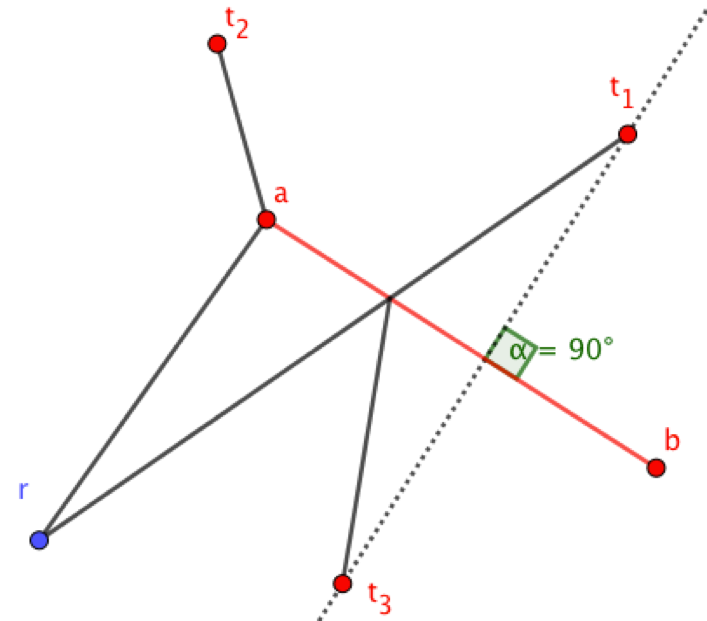
\includegraphics{pic/ef.png}
    \end{adjustbox}
\end{minipage}
\end{frame}

\begin{frame}{Multi-target Search: target heuristic}
\setbeamercovered{invisible}
\begin{minipage}{\textwidth}
\small{
When there are multiple targets ...
}
\onslide<2>{
    \begin{definition}{closest target of search node}
    is a target $t$ that $h_p(node, t)$ is minimal.
    \end{definition}
}
\end{minipage}%
\end{frame}

\begin{frame}{Multi-target Search: target heuristic}
\begin{minipage}{.4\textwidth}
\small{
    How to find the closest target for a search node?
}
\begin{itemize}
    \item<2-> \small{Let $NN_e$ be traditional nearest neighbor in euclidean space}
    \item<3-> \small{It must be:}
    \begin{itemize}
        \item<4-> $NN_e(areaA, a)$ or
        \item<5-> $NN_e(areaB, b)$ or
        \item<6-> $NN_e(areaC, r)$ or
        \item<7-> $NN_e(areaC', r')$ or
    \end{itemize}
    \item<8-> Standard \textit{R-tree} query
\end{itemize}

\end{minipage}%
\begin{minipage}{.6\textwidth}
    \begin{adjustbox}{max totalsize={.9\textwidth}{.9\textheight}, right}
    \centering
    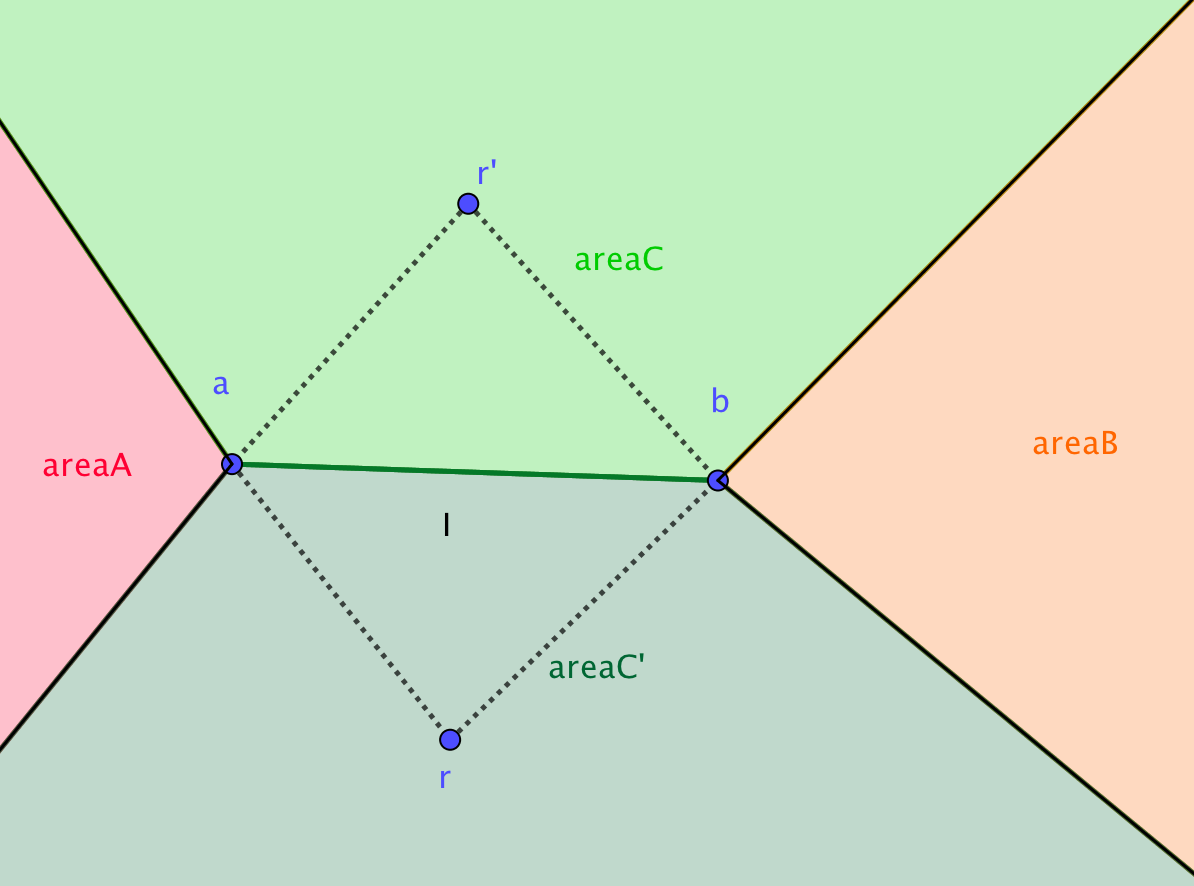
\includegraphics{pic/heuristic.png}
    \end{adjustbox}
\end{minipage}
\end{frame}

\begin{frame}{Multi-target Search: target heuristic}
\begin{minipage}{.9\textwidth}
\begin{itemize}
    \onslide<1-> \item \small{
        For each successor, assign the closest target to it
    }
    \onslide<2-> \item \small {
    Correctness:
    \begin{lemma}{Non-decreasing property:}
        Whenever the closest target of a search node changes,
        the \textit{h-value} never decrease.
    \end{lemma}
    }
\end{itemize}
\end{minipage}%
\end{frame}

\begin{frame}{Multi-target Search: target heuristic}
\setbeamercovered{invisible}
\begin{minipage}{.9\textwidth}
\begin{itemize}
    \item \small{Four \textit{R-tree} queries for each search  node is expensive}
    \item \small{So we are looking for further refinements...}
\end{itemize}
\end{minipage}%
\end{frame}

\begin{frame}{Multi-target Search: target heuristic refinements}
\setbeamercovered{invisible}
\begin{minipage}{.9\textwidth}
\begin{itemize}
    \item \small{Lazy query}
    \begin{Definition}
        In expansion, instead of finding a new target, successors can inherit the closest target from their parent if the \textit{h-value} doesn't change.
    \end{Definition}
    \item \small{Correctness}
    \begin{lemma}
        In this case, it is impossible to find a target with less \textit{h-value}.
    \end{lemma}
\end{itemize}
\end{minipage}%
\end{frame}

\begin{frame}{Multi-target Search: target heuristic refinements}
\setbeamercovered{invisible}
\begin{minipage}{.9\textwidth}
\begin{itemize}
    \item \small{Reassignment}
    \begin{definition}
        \small Once $t$ be retrieved, we must reassign another target to those search nodes who are regarding $t$ as their closest target
    \end{definition}
    \item \small{Lazy reassignment}
    \begin{definition}
        \small Instead of exploring the entire open list, we can do reassignment when such search node pop out
    \end{definition}
    \item \small{Correctness}
    \begin{lemma}
        \small Lazy reassignment doesn't change relative expansion order.
    \end{lemma}
\end{itemize}
\end{minipage}%
\end{frame}
\section{Experiments}
\begin{frame}{Benchmark Problem}
\begin{minipage}{.4\textwidth}
% \begin{itemize}
\small{Dataset in \textit{Zhang, EDBT 2004}: no longer available,
 so we generate new benchmark problems:}
\begin{itemize}
    \onslide<2-> \item \small{All parks ($\approx 9000$) in Australia from \textit{OpenStreetMap}}
    \onslide<3-> \item \small{Use them as polygonal obstacles}
\end{itemize}
% \end{itemize}
\end{minipage}%
\begin{minipage}{.6\textwidth}
    \begin{adjustbox}{max totalsize={.9\textwidth}{.9\textheight}, right}
    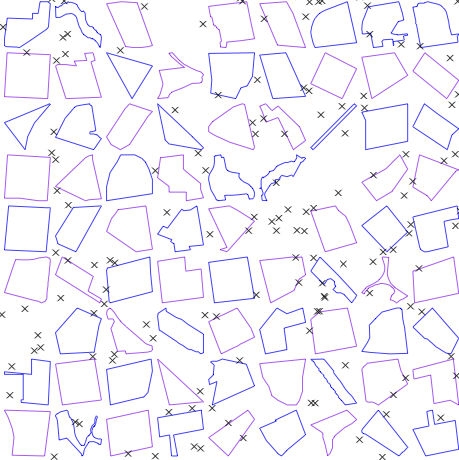
\includegraphics{pic/distribution.png}
    \end{adjustbox}
\end{minipage}
\end{frame}

\begin{frame}{Competitors}
\small{There are two types of test case:}
\begin{itemize}
    \item<1-> \small{Dense targets: $|T| \approx |O|, |O| \approx 9000$}
    \item<1-> \small{Sparse targets: $|T| <= 10, |O| \approx 9000$}
\end{itemize}
\small{In dense targets experiments, we compare between:}
\begin{itemize}
    \item<1-> \small{\textit{LVG} (from \textit{Zhang, EDBT 2004})}
    \item<1-> \small{Interval heuristic}
    \item<1-> \small{Target heuristic}
\end{itemize}
\small{In sparse targets experiments, we compare between:}
\begin{itemize}
    \item<1-> \small{burte-force Polyanya}
    \item<1-> \small{Interval heuristic}
    \item<1-> \small{Target heuristic}
\end{itemize}
\end{frame}

\begin{frame}{Dense targets}
\begin{minipage}{.5\textwidth}
    \centering
    $\scriptscriptstyle |O| \approx 9000, |T| \approx |O|, k=1$
    \begin{adjustbox}{max totalsize={.9\textwidth}{.9\textheight}, right}
    \centering
    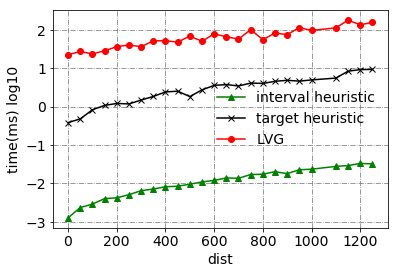
\includegraphics{pic/e1_dense_time.png}
    \end{adjustbox}
\end{minipage}%
\begin{minipage}{.5\textwidth}
    \centering
    $\scriptscriptstyle |O| \approx 9000, |T| \approx |O|, k \in [1, 10]$
    \begin{adjustbox}{max totalsize={.9\textwidth}{.9\textheight}, right}
    \centering
    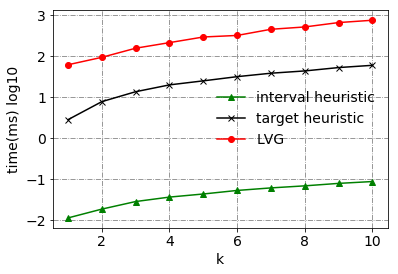
\includegraphics{pic/e2_dense_time.png}
    \end{adjustbox}
\end{minipage}
\begin{itemize}
    \item \small{\textit{Interval heuristic} is three order of magnitude faster than \textit{LVG}, in all aspects.}
\end{itemize}
\end{frame}

\begin{frame}{Sparse targets: fix $k=1$}
\centering
$\scriptscriptstyle |O| \approx 9000, |T| \in [1, 10]$
\begin{minipage}{.5\textwidth}
    \begin{adjustbox}{max totalsize={.9\textwidth}{.9\textheight}, right}
    \centering
    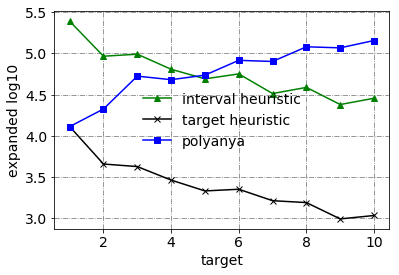
\includegraphics{pic/e3_gen.png}
    \end{adjustbox}
\end{minipage}%
\begin{minipage}{.5\textwidth}
    \begin{adjustbox}{max totalsize={.9\textwidth}{.9\textheight}, right}
    \centering
    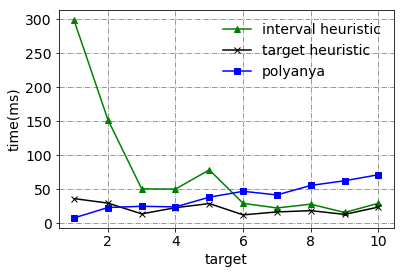
\includegraphics{pic/e3_time.png}
    \end{adjustbox}
\end{minipage}
\begin{itemize}
    \item \small{\textit{Target heuristic} always has smaller search space. (left)}
    \item \small{It gradually lose such advantage when $|T|$ increase. (right)}
    \item \small{Reason: the costly heuristic function.}
\end{itemize}
\end{frame}

\begin{frame}{Sparse targets: fix $|T|=10$}
\centering
$\scriptscriptstyle |O| \approx 9000, k \in [1, 10]$
\begin{minipage}{.5\textwidth}
    \begin{adjustbox}{max totalsize={.9\textwidth}{.9\textheight}, right}
    \centering
    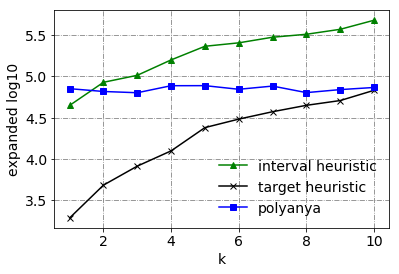
\includegraphics{pic/e2_sparse_gen.png}
    \end{adjustbox}
\end{minipage}%
\begin{minipage}{.5\textwidth}
    \begin{adjustbox}{max totalsize={.9\textwidth}{.9\textheight}, right}
    \centering
    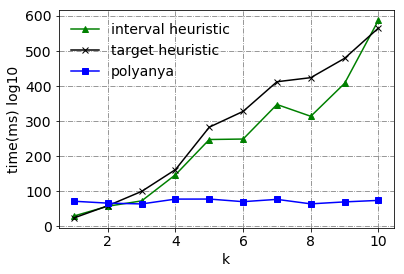
\includegraphics{pic/e2_sparse_time.png}
    \end{adjustbox}
\end{minipage}
\begin{itemize}
    \item \small{\textit{Target heuristic} always has small search space. (left)}
    \item \small{It always faster than \textit{Interval heuristic}. (right)}
    \item \small{It's outperformed by \textit{brute-force Polyanya} when $k>=2$. (right)}
    \item \small{Reason: lazy reassignment becomes more frequent.}
\end{itemize}
\end{frame}

\section{Conclusion and future work}
\begin{frame}{Conclusion}
    \begin{itemize}
        \item Proposed algorithms outcompte \textit{LVG} in all cases
        \item \textit{Interval heuristic} works well when targets are many
        \item \textit{Target heuristic} works well when targets are few and $k$ is also small
    \end{itemize}
\end{frame}

\begin{frame}{Future works 1: improve other query processing}
    \begin{itemize}
        \item \small{
            Proposed algorithms can be used to speed up other types of spatial query which need to compute obstacle distance, e.g. \textit{Obstacle Reverse Nearest Neighbor}.
        }
    \end{itemize}
\end{frame}

\begin{frame}{Future works 2: improve \textit{target heuristic}}
    \begin{itemize}
        \item \small {
          \textit{Target heuristic} cost $\approx 80\%$ of total run time in \textit{R-tree} query. 
        }
        \item \small {
            Improve it by combining four queries into one, or using more suitable datastructure.
        }
    \end{itemize}
\end{frame}

\begin{frame}{Future works 3: improve \textit{brute-force Polyanya}}
    \begin{itemize}
        \item \small {
            We notice that \textit{brute-force Polyanya} sometimes outcompetes proposed algorithms in sparse scenario.
        }
        \item \small {
            Instead of considering every targets, maybe a smart pruning strategy can make it work in general scenario. 
        }
    \end{itemize}
\end{frame}
\section{End}
\begin{frame}{End}
    \centering
    \Huge {Q \& A}
\end{frame}

\begin{frame}{End}
    \centering
    \Huge {Thank you!}
\end{frame}
% -----------------------------------------------------------------------------
\end{document}
%-----------------------------------------------
